\hfour{Architektur und ERD}

\begin{figure}[H]
    \centering
    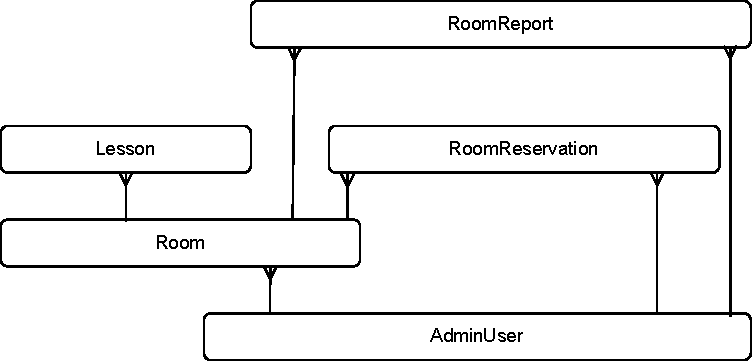
\includegraphics{media/MariaDB/ERD.svg.pdf}
    \caption{Entity Relationship Diagramm (ERD) des Projeks ZELIA}
\end{figure}

Die Architektur der Datenbank im Projekt \ZELIA\ ist so gewählt, dass die Daten, welche die Benutzer*innen eingeben oder auslesen wollen sicher und vor allem konsistent abgespeichert werden können. Die gesamte Datenbankstruktur besteht aus fünf Tabellen, welche in Beziehungen zueinander stehen.

\hfive{Tabelle AdminUser}

Die Tabelle, welche sich in der Hierarchie befindet ist die Tabelle "AdminUser". In ihr werden Benutzer angelegt, welche im "Admin-Dashboard" alle Meldungen oder Buchungen vorfinden und verwalten können. Außerdem werden in ihr verantwortliche Personen für gewisse Räume eingetragen.

\begin{figure}[H]
    \centering
    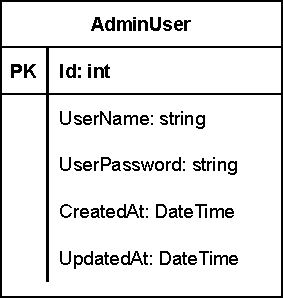
\includegraphics{media/MariaDB/AdminUser.svg.pdf}
    \caption{Spalten der Tabelle "AdminUser"}
\end{figure}

\hfive{Tabelle Room}

Eine Ebene weiter oben befindet sich eine der zentralsten Tabellen im gesamten Produkt, nämlich die Tabelle "Room". Sie enthält alle Räume und dazugehörige Infos zu ihnen (siehe Abbildung \ref{fig:RoomTableColls}). Wenn im ERD nach unten geblickt wird, hat sie eine Beziehung zur Tabelle AdminUser. Diese ist notwendig um einem Raum einen bestimmten "AdminUser" zuordnen zu können und um so den Überblick über die jeweilig verantwortliche Person zu behalten (Kardinalität 1:n).

\begin{figure}[H]
    \centering
    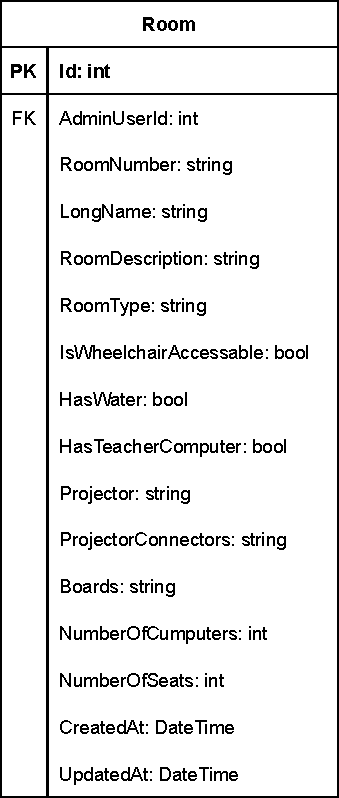
\includegraphics{media/MariaDB/Room.svg.pdf}
    \caption{Spalten der Tabelle "Room"}
    \label{fig:RoomTableColls}
\end{figure}

\hfive{Tabelle RoomReport}

Die Tabellen "RoomReport" ist für das Melden und Verwalten von Schäden in einem Raum zuständig. Deshalb ist jeder Meldungseintrag der Tabelle auch einem Raum zugeordnet und ein Raum kann mehrere Meldungen enthalten (Kardinalität 1:n). Außerdem hat die Tabelle "RoomReport" eine Beziehung zur Tabelle "AdminUser" um die verantwortliche Person für die Meldung zu bestimmen (Kardinalität 1:n). Welche Details zu einer Meldung angegeben werden müssen kann aus der Abbildung unten entnommen werden. Wichtig ist aber, dass der Status einer Meldung von der verantwortlichen Person geändert werden kann, je nachdem in welcher Phase sich die Meldung befindet. Außerdem wird die Email Adresse der Person vermerkt, damit nachverfolgbar bleibt wer welche Meldung aufgegeben hat.

\begin{figure}[H]
    \centering
    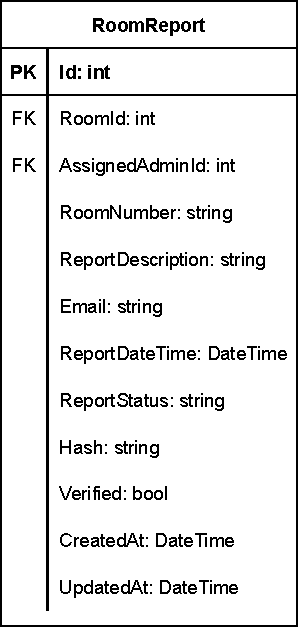
\includegraphics{media/MariaDB/RoomReport.svg.pdf}
    \caption{Spalten der Tabelle "RoomReport"}
\end{figure}

\hfive{Tabelle RoomReservation}

In der Tabelle "RoomReservation" werden alle Buchungen, welche über \ZELIA\ getätigt werden abgespeichert und verwaltet. Wie beim "RoomReport" hat auch diese Tabelle Beziehungen zu den Tabellen "AdminUser" und "Room" (jeweils die Kardinalität 1:n). Die Details können wieder aus der nachfolgenden Abbildung entnommen werden. Genauso wie in der Tabelle "RoomReport" kann der Status der Buchung geändert werden um der reservierenden Person zu sagen, ob eine Buchung möglich ist, oder nicht. Das System mit der E-Mail Zuordnung bleibt ebenfalls gleich wie in der oberen Tabelle beschrieben.

\begin{figure}[H]
    \centering
    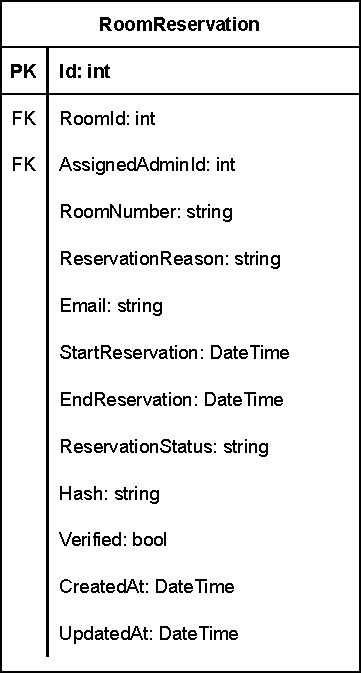
\includegraphics{media/MariaDB/RoomReservation.svg.pdf}
    \caption{Spalten der Tabelle "RoomReservation"}
\end{figure}

\hfive{Tabelle Lessons}

Die Tabelle "Lessons" kommt im aktuellen Projekt nicht zum Einsatz, ist jedoch für eine Erweiterung oder Umstrukturierung der Produktarchitektur mitimplementiert worden. Sollte beispielsweise einmal in regelmäßigen Abständen die Daten von "WebUntis" in diese Tabelle geschrieben werden sollen (Umstrukturierung des Cache), ist dies ohne eine Erweiterung des Datenbanksystems möglich. Sie enthält nur eine Beziehung zur Tabelle Room, um abzubilden in welchem Raum die aktuelle Stunde stattfindet. Die restlichen Spalteneinträge für eine Datensatz würden bei einer Verwendung der Tabelle von der API und "WebUntis" befüllt werden. Details zu dem Spaltenbezeichnungen können aus der Abbildung unten entnommen werden.

\begin{figure}[H]
    \centering
    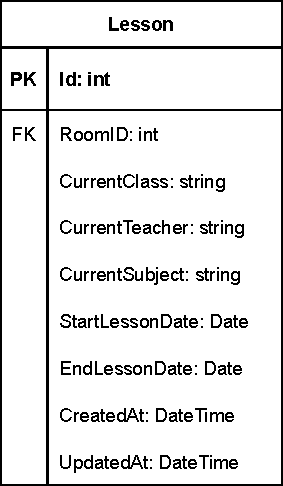
\includegraphics{media/MariaDB/Lesson.svg.pdf}
    \caption{Spalte der Tabelle "Lessons"}
\end{figure}
